\documentclass[../DS02.tex]{subfiles}%
\graphicspath{{./figures/}}%

\begin{document}%

\section[66]"P"{Étude d'une lampe de secours rechargeable\ifcorrige{~\small\textit{(D'après CCINP TSI 2022)}}}

\enonce{%
	Il est recommandé d'avoir sur soi une lampe pour être vu en cas de
	détresse ou tout simplement pour se déplacer par nuit noire. Pour ne pas
	avoir à gérer des piles défaillantes ou des accumulateurs non chargés,
	une «~lampe à secouer~» peut s'avérer utile. Un extrait d'une
	description publicitaire de cet objet est rapporté ci-dessous.

	\begin{tcn}(defi)"info"{Extrait d'une publicité pour une lampe à secouer}
		En secouant la lampe 30 secondes (un peu comme une bombe de peinture),
		de l'énergie électrique est produite et stockée dans un condensateur.
		Vous obtenez alors environ 20 minutes d'une lumière produite par une DEL
		(diode électroluminescente).

		Si vous n'utilisez pas toute l'énergie produite, elle restera stockée
		dans le condensateur pendant plusieurs semaines pour être ensuite
		immédiatement disponible sur simple pression du bouton marche/arrêt.
	\end{tcn}

	On part d'une situation où on suppose que le condensateur vient d'être
	chargé et que la tension à ses bornes est $U_0 = \SI{3.3}{V}$. On
	cesse alors d'agiter la lampe et donc de recharger le condensateur.

	\noindent
	\begin{minipage}[c]{.55\linewidth}
		Tout d'abord, on étudie la décharge de ce condensateur de capacité
		$C = \SI{10}{F}$ («~supercondensateur~») dans un conducteur
		ohmique de résistance $R$ pouvant modéliser une lampe à incandescence.
		Le circuit étudié est donc représenté par le schéma de la
		figure~\ref{fig:lampe1}. La partie de circuit utile lors de la phase de charge
		du condensateur n'est pas représentée.

		À l'instant initial $t = 0\ \mathrm{s}$, on ferme l'interrupteur K et
		la décharge commence.
	\end{minipage}
	\hfill
	\begin{minipage}[c]{.40\linewidth}
		\vspace{0pt}
		\begin{center}
			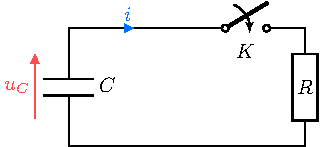
\includegraphics[width=.8\linewidth]{circuit_plain}
			\captionof{figure}{Circuit électrique équivalent lors de la phase de
				décharge du condensateur}
			\label{fig:lampe1}
		\end{center}
	\end{minipage}
}%

\QR[10]{%
	Établir l'équation différentielle vérifiée par $u_c(t)$ pendant la décharge
	en faisant apparaître une constante de temps $\tau$ dont on donnera
	l'expression. Puis déterminer l'expression littérale de la solution de cette
	équation différentielle.
}{%
	Avec une loi des mailles~:
	\begin{DispWithArrows*}
		u_C(t) - Ri(t) &\stm{=} 0
		\Arrow{%
			RCT C convention générateur\\
			$i = \boxed{-}C \dv{u_C}{t}$
		}%
		\\\Lra
		u_C(t) + RC \dv{u_C}{t} &\stm{=} 0
		\Arrow{Forme canonique et $\tau \stm{=} RC$}
		\\\Lra
		\dv{u_C}{t} + \frac{u_C(t)}{\tau} &\stm{=} 0
	\end{DispWithArrows*}
	\begin{isd}
		On résout en injectant la forme générique $u_C(t) \stm{=} K \exr^{rt}$~:
		\begin{align*}
			r \cdot \cancel{K\exr^{rt}} + \frac{\cancel{K\exr^{rt}}}{\tau} & = 0
			\\\Lra
			r                                                              & \stm{=} - \frac{1}{\tau}
		\end{align*}
		\tcblower
		Donc la forme générale de $u_C(t) \stm{=} K \exr^{-t/\tau}$. Or, $u_C(0^-) =
			U_0 = u_C(0^+)$ par continuité de la tension aux bornes de $C$ \pt{1}. Cela
		donne donc $U_0 = K$ \pt{1}, et ainsi
		\[
			\boxed{u_C(t) \stm{=} U_0 \exr^{-t/\tau}}
		\]
	\end{isd}
}%

% \enonce{%
% 	Au bout d'une durée environ égale à $5\tau$ on peut considérer que la
% 	décharge du condensateur est quasi-complète.
% }%

\QR[3]{%
	Si l'on considère que la décharge s'effectue en 20 minutes (comme
	précisé dans le document fourni), déterminer la valeur de la
	résistance $R$ du conducteur ohmique qu'il faut alors associer au
	condensateur de capacité $C = \SI{10}{F}$.
}{%
	La décharge d'un condensateur s'accomplit à $t_{99} \approx 5\tau = 5RC$ \pt{1}.
	Ainsi,
	\begin{gather*}
		5\tau = t_{99}
		\Lra
		RC = \frac{t_{99}}{5}
		\Lra
		\boxed{R \stm{=} \frac{t_{99}}{5C}}
		\qav
		\left\{
		\begin{array}{rcl}
			t_{99} & = & \SI{20}{minutes} = \SI{1200}{s}
			\\
			C      & = & \SI{10}{F}
		\end{array}
		\right.\\
		\AN
		\xul{
			R \stm{=} \SI{24}{\ohm}
		}
	\end{gather*}
}%

\enonce{%
	Certains modèles électriques plus élaborés du «~supercondensateur~»
	utilisé ici permettent de traduire, plus fidèlement à la réalité, son
	comportement réel dans un circuit. Un des modèles possibles fait
	apparaître, autour de la capacité $C$, une résistance $R_f$ en
	parallèle et une résistance série $R_s$ conformément au schéma de la
	figure~\ref{fig:lampe2}.

	\begin{figure}[htbp!]
		\centering
		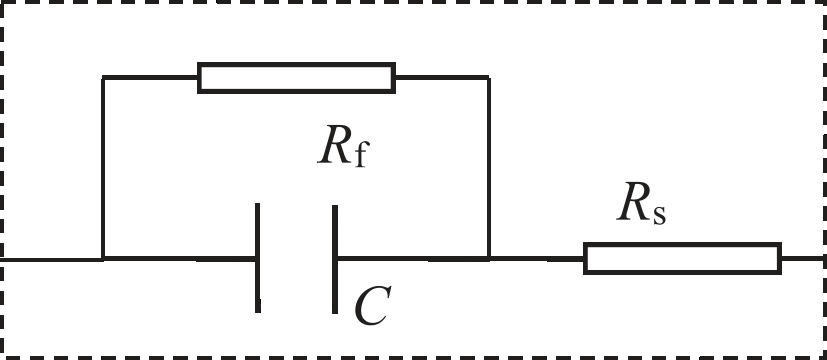
\includegraphics[width=5cm]{supercondo}
		\caption{Modèle plus fidèle à la réalité pour le «~supercondensateur~»}
		\label{fig:lampe2}
	\end{figure}
}%

\QR[4]{%
	Pour quelles valeurs limites de $R_s$ et $R_f$ retrouve-t-on le modèle
	simple ($C$ seul) du «~supercondensateur~»?
}{%
	Avec $R_f \to \infty$ \pt{1}, on a un interrupteur ouvert \pt{1}, et avec $R_s
		= 0$ \pt{1} on a un fil \pt{1}, ce qui correspond bien à une capacité idéale
	seule.
}%

\enonce{%
	Pour la suite des questions, on revient au modèle simple ($C$ seul)
	pour le condensateur, toujours initialement chargé sous une tension
	$U_0 = \SI{3.3}{V}$.

	On remplace maintenant le conducteur ohmique de résistance $R$ par une
	DEL dont les caractéristiques sont les suivantes (Figure~\ref{fig:lampe3} et
	Tableau~\ref{tab:lampe})~:

	\begin{figure}[htbp!]
		\centering
		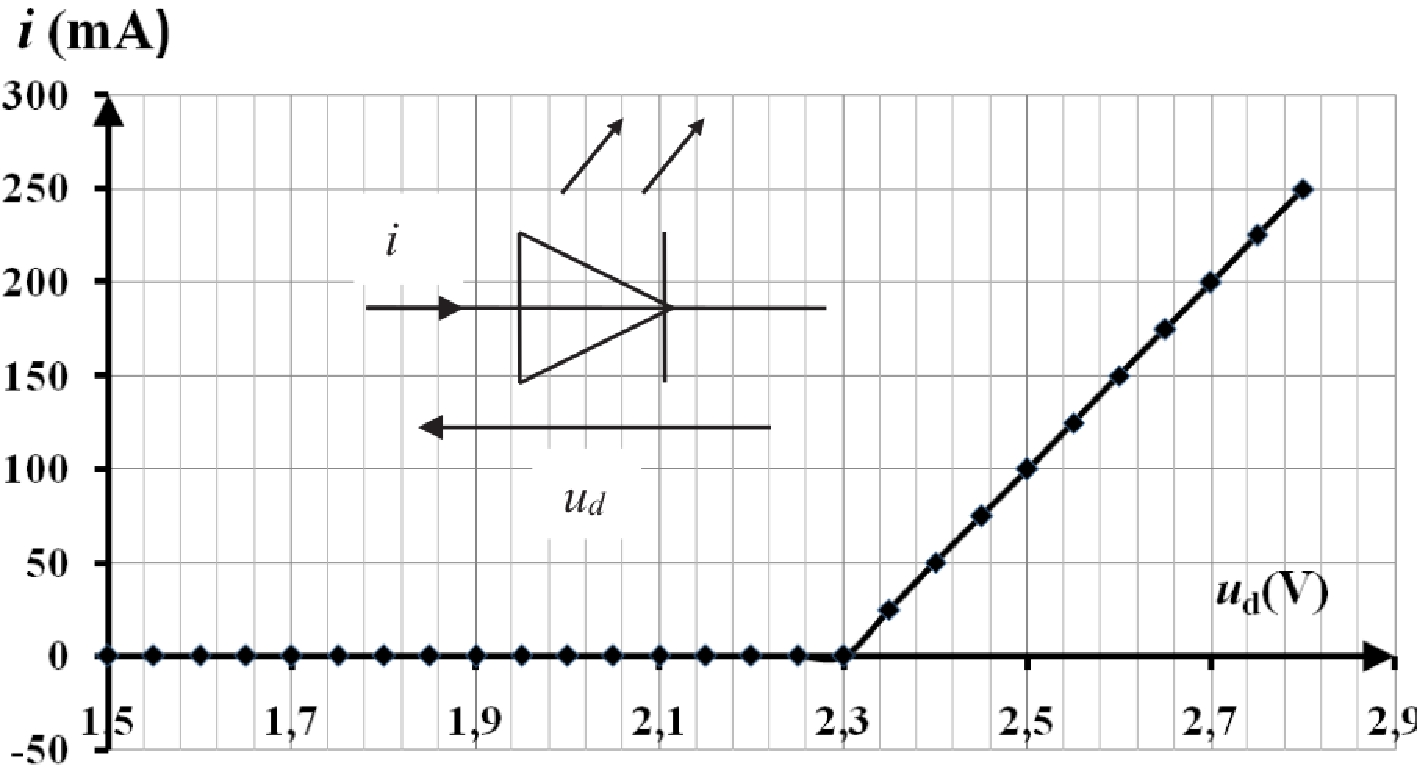
\includegraphics[scale=1]{led_carac}
		\caption{Caractéristique $i=f(u_d)$ et symbole pour la diode
			électroluminescente DEL.}
		\label{fig:lampe3}
	\end{figure}

	% \begin{figure}
	% 	\centering
	% 	\includegraphics[width=14cm,height=\textheight]{images-DS2/pb-lampe-fig4.pdf}
	% 	\caption{}\label{fig:lampe4}
	% \end{figure}

	\begin{table}[htbp!]
		\centering
		\caption{Electrical \& Optical Characteristics}
		\begin{tabular}{ccccccc}
			\toprule
			\textbf{Parameter}       &
			\textbf{Symbol}          &
			\textbf{Condition}       &
			\textbf{Min.}            &
			\textbf{Typ.}            &
			\textbf{Max.}            &
			\textbf{Unit}
			\\
			\midrule
			Luminous Flux            &
			$\Phi_V$                 &
			$i = \SI{200}{mA}$       &
			6                        &
			8.5                      &
			--                       &
			\si{lm}
			\\
			Forward Voltage          &
			$u_d$                    &
			$i = \SI{200}{mA}$       &
			--                       &
			2.5                      &
			2.8                      &
			\si{V}
			\\
			D.C. Forward Current Max &
			$i_M$                    & --                 & -- & --  & 250 & \si{mA}
			\\
			Peak Wavelength          &
			$\lambda_p$              & $i = \SI{200}{mA}$ & -- & 635 & --  & \si{nm}
			\\
			Dominant Wavelength      &
			$\lambda_d$              & $i = \SI{200}{mA}$ & -- & 624 & --  & \si{nm}
			\\
			Reverse Current          &
			$i_r$                    & $u_r = \SI{5}{V}$  & -- & --  & 50  & \si{\micro A}
			\\
			Viewing angle            &
			$2\Phi_{1/2}$            & $i = \SI{200}{mA}$ & -- & 120 & --  & \si{deg}
			\\
			Spectrum Line Halfwidth  &
			$\Delta{\lambda}$        & $i = \SI{200}{mA}$ & -- & 20  & --  & \si{nm}
			\\
			\bottomrule
		\end{tabular}
		\label{tab:lampe}
	\end{table}

	Pour cette diode, on appelle tension seuil, notée $U_S$ la tension
	minimale au-delà de laquelle la diode devient passante. On convient
	alors que la diode électroluminescente cesse d'émettre suffisamment de
	lumière dès que $u_d < U_S + \SI{0.1}{V}$.
}%

\QR[14]{%
	Par quel dipôle peut-on modéliser la DEL lorsqu'elle est bloquée (\(u_d <
	\SI{2.3}{V}\))~?. D'autre part, lorsqu'elle est passante ($u_d >
		\SI{2.3}{V}$), déterminer l'équation de la caractéristique $i(u_d)$ en
	donnant les valeurs numériques. Proposer alors un modèle électrique équivalent
	sous forme d'un générateur de \textsc{Thévenin}. On fera le schéma électrique
	correspondant en précisant bien les sens de l'intensité de la tension $u_d$.
}{%
	\ifstudent{%
		\smallbreak
		\vspace{-25pt}
	}%
	\begin{itemize}
		\item Lorsque la DEL est bloquée, on a $i = 0$ \pt{1} et c'est donc un
		      \textbf{interrupteur ouvert} \pt{1}.
		\item Lorsqu'elle est passante, on a une caractéristique affine, d'équation
		      \[
			      i \stm{=} a u_d + b
		      \]
		      \begin{isd}
			      \begin{itemize}
				      \item $a$ est le coefficient directeur~:
				            \begin{gather*}
					            \boxed{
						            a \stm{=} \frac{i\ind{max} - i\ind{min}}{u_{d,\rm max} -
							            u_{d,\rm lim}}
					            }
					            \qav
					            \left\{
					            \begin{array}{rcl}
						            i\ind{max}    & = & \SI{250}{mA}
						            \\
						                          & = & \SI{0.250}{A}
						            \\
						            i\ind{min}    & = & 0
						            \\
						            u_{d,\rm max} & = & \SI{2.8}{V}
						            \\
						            u_{d,\rm lim} & = & \SI{2.3}{V}
					            \end{array}
					            \right.\\
					            \AN \xul{
						            a \stm{=} \SI{0.50}{S}
					            }
				            \end{gather*}
			      \end{itemize}
			      \tcblower
			      \begin{itemize}
				      \item $b$ est l'ordonnée à l'origine, que l'on obtient en
				            connaissant les coordonnées d'un point. Ici, pour le point
				            limite de blocage, on a
				            \begin{gather*}
					            \underbracket[1pt]{i\ind{lim}}_{=0} = a u_{d,\rm lim} + b
					            \Lra
					            \boxed{b \stm{=} -a u_{d,\rm lim}}
					            \\
					            \AN
					            \xul{b \stm{=} \SI{-1.15}{A}}
				            \end{gather*}
			      \end{itemize}
		      \end{isd}
		      Pour la modéliser en générateur de \textsc{Thévenin}, il faut écrire
		      sa
		      caractéristique sous la forme $u_d = ri + U_S$ \pt{1}~; on l'isole de
		      l'équation précédente puis on détermine $a'$ et $b'$ en fonction des
		      données précédemment trouvées~:
		      \smallbreak
		      \begin{isd}
			      \begin{gather*}
				      i = a u_d + b
				      \Lra
				      au_d = i - b
				      \Lra
				      \boxed{u_d \stm{=} \frac{1}{a}i + \frac{-b}{a}}
				      \\\beforetext{donc}
				      \boxed{r = \frac{1}{a}}
				      \qet
				      \boxed{U_s = \frac{-b}{a}}
				      \\\AN
				      \xul{r \stm{=} \SI{2}{\ohm}}
				      \qet
				      \xul{U_s \stm{=} \SI{2.3}{V}}
			      \end{gather*}
			      \tcblower
			      D'où le schéma équivalent Figure~\ref{fig:del_thev}.
			      \begin{center}
				      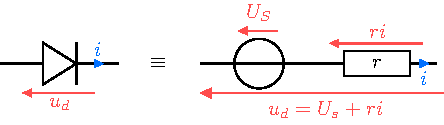
\includegraphics[scale=1]{diode_thevenin}
				      \captionof{figure}{\protect\pt{1}+\protect\pt{1}}
				      \label{fig:del_thev}
			      \end{center}
		      \end{isd}
	\end{itemize}
}%

\QR[6]{\label{q:diffeqcircdel}%
	Faire le schéma électrique de la DEL modélisée et insérée dans le
	circuit précédent. Puis, montrer que la nouvelle équation
	différentielle régissant l'évolution de $u_c(t)$ lorsque le
	condensateur se décharge dans la diode électroluminescente est
	$\DS\dv{u_c}{t} + \dfrac{u_c(t)}{\tau'} = \dfrac{U_S}{\tau'}$.
	Préciser l'expression de $\tau'$.
}{\label{q:diffeqcircdel}%
	\ifstudent{%
		\smallbreak
		\vspace{-25pt}
	}%
	\noindent
	\begin{minipage}[c]{.40\linewidth}
		\begin{center}
			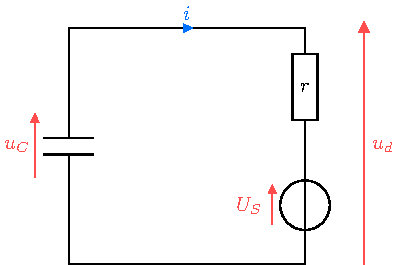
\includegraphics[scale=1]{circuit_diode_thev}
			\captionof{figure}{Schéma équivalent \protect\pt{1}+\protect\pt{1}}
			\label{fig:circ_del_thev}
		\end{center}
	\end{minipage}
	\hfill
	\begin{minipage}[c]{.60\linewidth}
		\begin{DispWithArrows*}[fleqn, mathindent=30pt]
			u_C - ri - U_S &\stm{=} 0
			\Arrow{RCT C conv.\ géné.}
			\\\Lra
			u_C + rC \dv{u_C}{t} &\stm{=} U_S
			\Arrow{Canonique et $\tau' \stm{=} rC$}
			\\\Lra
			\dv{u_C}{t} + \frac{u_C(t)}{\tau'} &\stm{=} \frac{U_S}{\tau'}
		\end{DispWithArrows*}
	\end{minipage}
}%

\QR[8]{%
	Déterminer la solution $u_c(t)$ de cette nouvelle équation
	différentielle, avec les mêmes conditions initiales que précédemment,
	puis représenter graphiquement l'allure de son évolution en fonction
	du temps, en mettant en évidence les points importants du graphe
	(valeur et tangente à l'origine ainsi qu'une asymptote éventuelle).
}{%
	\ifstudent{%
		\smallbreak
		\vspace{-25pt}
	}%
	\noindent
	\begin{minipage}[c]{.70\linewidth}
		On trouve comme précédemment une solution homogène de la forme
		$\boxed{u_{C,h}(t) = B \exr^{-t/\tau'}}$ \pt{1}. La solution particulière
		constante donne $\boxed{u_{C,p}(t) = U_S}$ \pt{1}. D'où la solution générale
		totale~:
		\[
			u_C(t) \stm{=} u_{C,h}(t) + u_{C,p} = B\exr^{-t/\tau'} + U_S
		\]
		On a toujours $u_C(0) = U_0$, soit ici
		\[
			U_0 = B + U_S
			\Lra
			\boxed{B \stm{=} U_0 - U_S}
		\]
		\[
			\Ra
			\boxed{u_{C}(t) \stm{=} U_S + (U_0 - U_S)\exr^{-t/\tau'}}
			\qav
			\boxed{\tau' = rC}
		\]
	\end{minipage}
	\hfill
	\begin{minipage}[c]{.25\linewidth}
		\begin{center}
			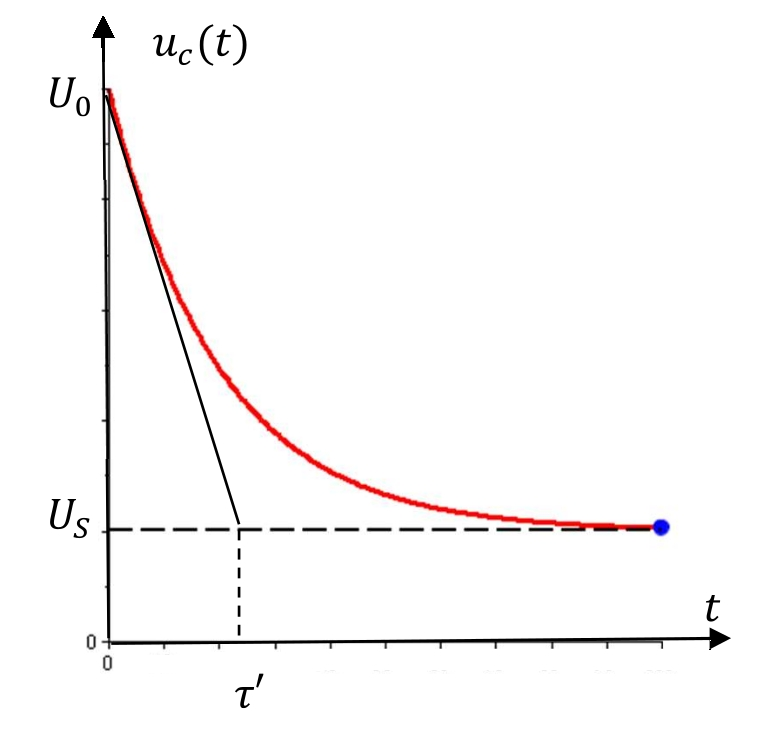
\includegraphics[width=\linewidth]{uct}
			\captionof{figure}{\protect\pt{1}+\protect\pt{1}+\protect\pt{1}}
		\end{center}
	\end{minipage}
}%

\QR[5]{%
	Déterminer l'expression littérale de $i(t)$, puis représenter
	graphiquement l'allure de son évolution en fonction du temps, en
	mettant en évidence les points importants.
}{%
	\ifstudent{%
		\smallbreak
		\vspace{-25pt}
	}
	\noindent
	\begin{minipage}[c]{.70\linewidth}
		Avec la RCT de C en convention générateur~:
		\begin{gather*}
			i \stm{=} -C \dv{u_C}{t}
			\Lra
			i = -C \left( -\frac{1}{\tau'} \right)(U_0 - U_S)\exr^{-t/\tau'}
			\\\Lra
			\boxed{i(t) \stm{=} \frac{U_0-U_S}{r}\exr^{-t/\tau'}}
		\end{gather*}
	\end{minipage}
	\hfill
	\begin{minipage}[c]{.25\linewidth}
		\begin{center}
			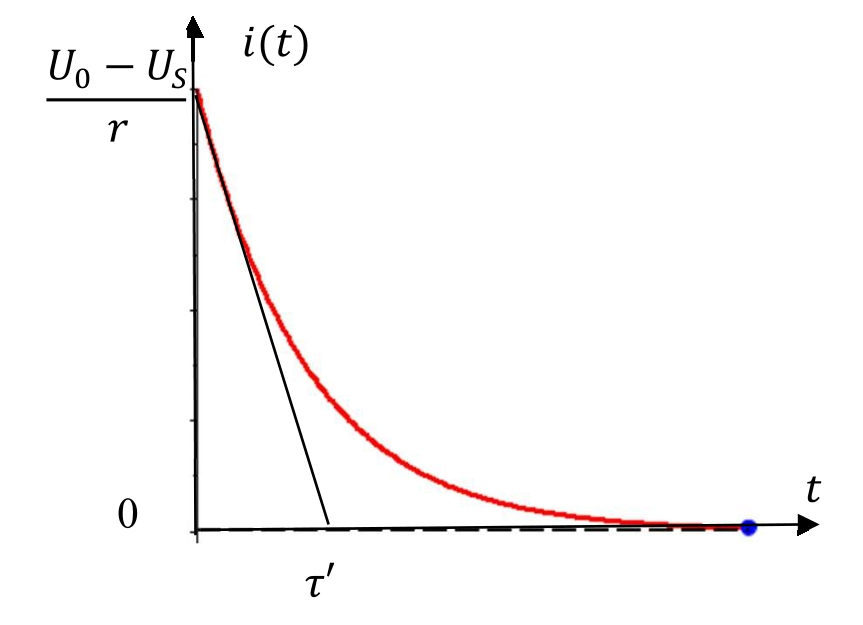
\includegraphics[width=\linewidth]{it}
			\captionof{figure}{\protect\pt{1}+\protect\pt{1}+\protect\pt{1}}
		\end{center}
	\end{minipage}
}%

\QR[6]{%
	À l'aide des caractéristiques techniques fournies dans le
	Tableau~\ref{tab:lampe}, indiquer si le fonctionnement correct de la DEL est
	garanti sans dommage. Proposer une solution pour éventuellement remédier au
	problème rencontré.
}{%
	On remarque que $u_{C,\rm max} = U_0 = \SI{3.3}{V}$ \pt{1} et que $i\ind{max}
		= \frac{U_0 - U_S}{r} = \SI{0.5}{A}$. \pt{1}
	\smallbreak
	Or, d'après le Tableau donné, $i\ind{max} = \SI{250}{mA}$ \pt{1} et
	$u_{c,\rm
				max} = \SI{2.8}{V}$. \pt{1}
	\smallbreak
	Ainsi, il faut restreindre la charge initiale du condensateur en
	\textbf{secouant moins longtemps} \pt{1} ($\approx \SI{20}{s}$). On peut aussi
	\textbf{ajouter une résistance en série} \pt{1} avec la DEL pour diviser la
	valeur initiale de l'intensité.
}%

\QR[7]{%
	Prévoir, sans la mise en œuvre de la solution précédente, la durée
	approximative d'éclairage de cette lampe notée $T$ (on rappelle que
	$\ln(10) \approx \num{2.3}$). Conclure.
}{%
	D'après l'énoncé, la lampe éclaire tant que $u_d > U_s + \SI{0.1}{V}$ \pt{1}~;
	or, d'après le schéma de la question~\ref{q:diffeqcircdel}, $u_d = u_C$
	\pt{1}. La condition d'éclairage est donc
	\begin{DispWithArrows*}[groups]
		\cancel{U_S} + (U_0 - U_S)\exr^{-t/\tau'} &\stm{>} \cancel{U_S} + \SI{0.1}{V}
		\Arrow{$T$ la limite}
		\\\Ra
		(U_0 - U_S)\exr^{-T/\tau'} &= \SI{0.1}{V}
		\\\Lra
		\exr^{-T/\tau'} &= \frac{\SI{0.1}{V}}{U_0 - U_S}
		\CArrow{$\ln (\cdot )$}
		\\\Lra
		\frac{-T}{\tau'} &\stm{=} \ln \frac{\SI{0.1}{V}}{U_0 - U_S}
		\\\Lra
		\Aboxed{T &\stm{=} \tau' \ln \frac{U_0 - U_S}{\SI{0.1}{V}}}
		\qav
		\left\{
		\begin{array}{rcl}
			\tau'     & = & rC
			\\
			r         & = & \SI{2}{\ohm}
			\\
			C         & = & \SI{10}{F}
			\\
			U_0 - U_S & = & \SI{1.0}{V}
		\end{array}
		\right.\\
		\AN
		\makebox[0pt][l]{$\xul{\phantom{T \approx \SI{46}{s}}}$}
		T &\stm{\approx} \SI{46}{s}
	\end{DispWithArrows*}
	On est \textbf{très loin des \SI{20}{minutes} annoncées}~! \pt{1}
}%

\QR[3]{%
	Exprimer, en fonction de $U_0$ et de
	$U_{f} = U_S + \SI{0.1}{V}$, le pourcentage d'énergie restante
	dans le condensateur lorsque la DEL cesse d'émettre de la lumière par
	rapport à l'énergie initiale accumulée (on ne cherche pas à la
	calculer, mais on estime ici ce pourcentage à environ 50 \%).
}{%
	\vspace{-25pt}
	\begin{gather*}
		\beforetext{On a}
		\Ec_C(t) \stm{=} \frac{1}{2}C u_C(t)^2
		\\\Ra
		\Ec_{C,i} = \frac{1}{2}C U_0{}^2
		\qet
		\Ec_{C,f} = \frac{1}{2}C U_f{}^2
		\\\Ra
		p \stm{=} 100 \times \frac{\Ec_{C,f}}{\Ec_{c,i}}
		\Lra
		\boxed{p \stm{=} 100 \times \frac{U_f{}^2}{U_0{}^2}}
	\end{gather*}
}%

\end{document}
